
\begin{flushleft}
	
	\begin{enumerate}
		\item \textbf{whoami}: Display username who is logged in.
		\newline
		Eg:
		\begin{tcolorbox}[breakable,notitle,boxrule=-0pt,colback=black,colframe=black]
			\color{green}
			\# whoami
			\newline
			\color{white}
			jack
		\end{tcolorbox}
		\bigskip
		\bigskip
		
		\item \textbf{users}: Display all the username who are currently logged in.
		\newline
		Eg:
		\begin{tcolorbox}[breakable,notitle,boxrule=-0pt,colback=black,colframe=black]
			\color{green}
			\# users
			\newline
			\fontdimen2\font=1em
			\color{white}
			jack jill lavatech
			\fontdimen2\font=4pt
		\end{tcolorbox}
		
		\bigskip
		
		\item \textbf{who}: Displays users currently logged with more details.
		\newline
		Eg:
		\begin{tcolorbox}[breakable,notitle,boxrule=-0pt,colback=black,colframe=black]
			\color{green}
			\# who
			\newline
			\color{white}
			\fontdimen2\font=1em
			jack   :0           2022-02-02 14:21 (:0)
			\newline
			jill :1           2022-02-03 13:52 (:1)
			\newline
			lavatech pts/0  2022-02-03 14:03 (192.168.0.105)
			\fontdimen2\font=4pt
		\end{tcolorbox}				
		Output explaination:
			\begin{itemize}
				\item Column 1 - Login name
				\item Column 2 - Login device (TTY or pts)
				\item Column 3 - Login date
				\item Column 4 - Login time 
				\item Column 5 - Local device or remote IP address from where the user is logged in
			\end{itemize}
		\bigskip
		\begin{tcolorbox}[breakable,notitle,boxrule=-0pt,colback=yellow,colframe=yellow]
			\color{black}
			\textbf{Note:} 
			\begin{itemize}
				\item TTY stands for \textbf{teletypewriter}: It is an input device that allows alphanumeric character to be typed in and sent to a computer.
				\item The pts/0 is telling which \textbf{"pseudo terminal"} the user is logged in on. 
			\end{itemize}
		\end{tcolorbox}
		Options with \textbf{who} command:
		\begin{itemize}
			\item \textbf{-H}: Prints the column headers.
			\newline
			Eg:
			\begin{tcolorbox}[breakable,notitle,boxrule=-0pt,colback=black,colframe=black]
				\color{green}
				\$ who -H 
			\end{tcolorbox}
			\item \textbf{-b}: Display the time and date of the last reboot.
			\newline
			Eg:
			\begin{tcolorbox}[breakable,notitle,boxrule=-0pt,colback=black,colframe=black]
				\color{green}
				\# who -b
			\end{tcolorbox}
		\end{itemize}
		\bigskip
		\item \textbf{w}: Shows who is logged and what they are doing.
			\newline
			Eg:
			\begin{tcolorbox}[breakable,notitle,boxrule=-0pt,colback=black,colframe=black]
				\color{green}
				\# w
				\color{white}
				\small
				\fontdimen2\font=1em
				\newline
				14:27:00 up 1 day, 5 min,  2 users,  load average: 1.86, 2.44, 2.70
				\newline
				\fontdimen2\font=1.2em
				USER     TTY      FROM             LOGIN@   IDLE   JCPU   PCPU WHAT
				\newline
				jack   :0       :0               Wed14   ?xdm?  14:25m  0.03s /usr/lib/g
				\newline
				lavatech :1       :1               13:52   ?xdm?  14:25m  0.00s /usr/lib/g
				\newline
				\fontdimen2\font=4pt
			\end{tcolorbox}
			
			Output explaination:
			\begin{itemize}
				\item Line 1 - Shows below details:
				\begin{itemize}
					\item Current time
					\item How long the system has been running.
					\item How many users are currently logged in.
					\item System load averages for the past 1, 5, and 15 minutes.
				\end{itemize}
				\item Line 2 - Header
				\item Line 3 - Login name, the tty name, the remote host, login time, idle time, JCPU, PCPU, and the command line of their current process.
			\end{itemize}
			\bigskip
			\bigskip
			\textbf{JCPU} - Time used by all processes attached to the tty.
			\newline
			\textbf{PCPU} - Time used by the current process, named in the "what" field.
		\bigskip
		\item \textbf{uname}: Displays the name of OS.
		\newline
		Eg:
		\begin{tcolorbox}[breakable,notitle,boxrule=-0pt,colback=black,colframe=black]
			\color{green}
			\fontdimen2\font=1em
			\# uname
			\newline
			\color{white}
			Linux
			\fontdimen2\font=4pt
		\end{tcolorbox}
		Options with \textbf{uname} command:
		\begin{itemize}
			\item \textbf{-r}: Displays the current release of OS.
			\newline
			Eg:
			\begin{tcolorbox}[breakable,notitle,boxrule=-0pt,colback=black,colframe=black]
				\color{green}
				\fontdimen2\font=1em
				\# uname -r
				\color{white}
				\newline
				3.6.18-194.el8
				\fontdimen2\font=4pt
			\end{tcolorbox}
			\item \textbf{-a}: Displays:
			\begin{itemize}
				\item Kernel name 
				\item System name 
				\item Kernel release
				\item Kernel version
				\item Machine processor 
				\item Hardware platform
			\end{itemize} 
			Eg:
			\begin{tcolorbox}[breakable,notitle,boxrule=-0pt,colback=black,colframe=black]
				\color{green}
				\fontdimen2\font=1em
				\# uname -a
				\color{white}
				\newline
				Linux lavatech 5.13.0-27-generic \#29~20.04.1-Ubuntu SMP Fri Jan 14 00:32:30 UTC 2022 x86\_64 x86\_64 x86\_64 GNU/Linux
				\fontdimen2\font=4pt
			\end{tcolorbox}
			\item \textbf{-n}: Prints the hostname of machine.
			\newline
			Eg:
			\begin{tcolorbox}[breakable,notitle,boxrule=-0pt,colback=black,colframe=black]
				\color{green}
				\fontdimen2\font=1em
				\# uname -n
				\fontdimen2\font=4pt
			\end{tcolorbox}
		\end{itemize}
		\bigskip
		
		\item \textbf{uptime}: Display belows details in one line:
		\begin{itemize}
			\item Current time
			\item How long the system has been running
			\item How many users are currently logged in
			\item System load averages for the past 1, 5, and 15 minutes
		\end{itemize}
		Eg:
		\begin{tcolorbox}[breakable,notitle,boxrule=-0pt,colback=black,colframe=black]
			\color{green}
			\fontdimen2\font=1em
			\# uptime
			\newline
			\color{white}
			 14:48:33 up 1 day, 27 min,  2 users,  load average: 2.58, 2.60, 2.76
			\fontdimen2\font=4pt
		\end{tcolorbox}
		\bigskip
		\bigskip
		\item \textbf{timedatectl}: Control the system time and date
		\bigskip
		\begin{tcolorbox}[breakable,notitle,boxrule=-0pt,colback=pink,colframe=pink]
			\color{black}
			\fontdimen2\font=1em
			Syntax: timedatectl [options] [arguments]
			\fontdimen2\font=4pt
		\end{tcolorbox}
		Eg:
		\begin{figure}[h!]
			\centering
			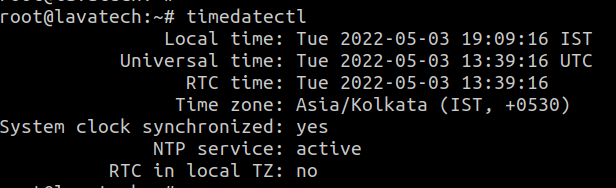
\includegraphics[scale=.45]{content/chapter2/images/timedate.png}
			\caption{Sample output}
			\label{fig:path25}
		\end{figure}
		\newline	
		Options with \textbf{timedatectl} command:
		\begin{itemize}
			\item \textbf{list-timezones}: Displays all available timezones.
			\newline
			Eg:
			\begin{tcolorbox}[breakable,notitle,boxrule=-0pt,colback=black,colframe=black]
				\color{green}
				\fontdimen2\font=1em
				\# timedatectl list-timezones
				\fontdimen2\font=4pt
			\end{tcolorbox}
			\item \textbf{set-timezone}: Sets timezone.
			\newline
			Eg:
			\begin{tcolorbox}[breakable,notitle,boxrule=-0pt,colback=black,colframe=black]
				\color{green}
				\fontdimen2\font=1em
				\# timedatectl set-timezone America/Jamaica
				\fontdimen2\font=4pt
			\end{tcolorbox}
		\end{itemize}	
		\bigskip
		\bigskip
		\item \textbf{date}: Display or set the date.
		\begin{enumerate}[label=(\alph*)]
			\item To display the date:
			\newline
			Eg:
			\begin{tcolorbox}[breakable,notitle,boxrule=-0pt,colback=black,colframe=black]
				\color{green}
				\fontdimen2\font=1em
				\# date
				\newline
				\color{white}
				Saturday 30 April 2022 12:24:24 PM IST
				\fontdimen2\font=4pt
			\end{tcolorbox}
			\item To set the date, the format is:
			\bigskip
			\begin{tcolorbox}[breakable,notitle,boxrule=1pt,colback=pink,colframe=pink]
				\color{black}
				\fontdimen2\font=1em
				Syntax: date "+\%formatters"
				\fontdimen2\font=4pt
			\end{tcolorbox}
			Eg:
			\bigskip
			\begin{tcolorbox}[breakable,notitle,boxrule=-0pt,colback=black,colframe=black]
				\color{green}
				\fontdimen2\font=1em
				\# date '+\%a \%h \%d \%T'
				\fontdimen2\font=4pt
			\end{tcolorbox}
		
			Valid date formatters:
			\newline
			\newline
			\begin{tabulary}{1.0\textwidth}{|p{8em}|p{16em}|}
				\toprule
				\textbf{Date Formatter} & \textbf{Description}\\
				\midrule
				\%m & month of year (01-12) \\
				\hline
				\%n & prints output to new line \\
				\hline
				\%d & day of month (01-31) \\
				\hline
				\%y & last two digits of year (00-99) \\
				\hline
				\%D & date as mm/dd/yy \\
				\hline
				\%H & hour (00-23) \\
				\hline
				\%M & minute (00-59) \\
				\hline
				\%S & second (00-59) \\
				\hline
				\%T & time as HH:MM:SS \\
				\hline
				\%j & day of year (001-366) \\
				\hline
				\%w & day of week (0-6) Sunday is 0 \\
				\hline
				\%a & abbreviated weekday (Sun-Sat) \\
				\hline
				\%h & abbreviated month (Jan-Dec) \\
				\hline
				\%r & 12-hour time w/ AM/PM (e.g., "03:59:42 PM")\\
				\bottomrule
			\end{tabulary}
		
			Options with \textbf{date} command:
			
			\begin{itemize}
				\item \textbf{-s datestring}: Sets the time and date to the value specified in the datestring only if you are root user.
				\newline
				Eg:
				\bigskip
				\begin{tcolorbox}[breakable,notitle,boxrule=-0pt,colback=black,colframe=black]
					\color{green}
					\fontdimen2\font=1em
					\# date -s '11/20/2003 12:48:00'
					\fontdimen2\font=4pt
				\end{tcolorbox}
				\item \textbf{-d datestring}: Display the specified date instead of actual current system date.
				\newline
				Eg:
				\bigskip
				\begin{tcolorbox}[breakable,notitle,boxrule=-0pt,colback=black,colframe=black]
					\color{green}
					\fontdimen2\font=1em
					\# date -d "last friday"
					\newline
					\# date -d "next friday"
					\newline
					\# date -d "yesterday"
					\fontdimen2\font=4pt
				\end{tcolorbox}
			\end{itemize}
			
		\end{enumerate}
		\bigskip
		\bigskip
		\item \textbf{cal}: Prints a calendar for the current month.
			\bigskip
			\begin{tcolorbox}[breakable,notitle,boxrule=-0pt,colback=pink,colframe=pink]
				\color{black}
				\fontdimen2\font=1em
				Syntax: cal [options] [[month] year]
				\fontdimen2\font=4pt
			\end{tcolorbox}
			Options with \textbf{cal} command:
			\begin{itemize}
				\item \textbf{-j}: Display julian dates (days numbered 1 to 365, starting from January 1).
				\newline
				Eg: To display calender for month-12 and year-2022 with julian dates.
				\begin{tcolorbox}[breakable,notitle,boxrule=-0pt,colback=black,colframe=black]
					\color{green}
					\fontdimen2\font=1em
					\# cal -j 12 2022
					\fontdimen2\font=4pt
				\end{tcolorbox}
				
				\begin{figure}[h!]
					\centering
					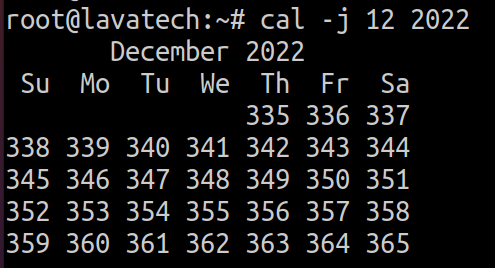
\includegraphics[scale=0.4]{content/chapter2/images/cal1.png}
					\caption{Sample output}
					\label{fig:cal1}
				\end{figure}

				\item \textbf{-m}: Display specific month.
				\newline
				Eg: To display calender of month-12.
				\begin{tcolorbox}[breakable,notitle,boxrule=-0pt,colback=black,colframe=black]
					\color{green}
					\fontdimen2\font=1em
					\# cal -m 12
					\fontdimen2\font=4pt
				\end{tcolorbox}
				
				\begin{figure}[h!]
					\centering
					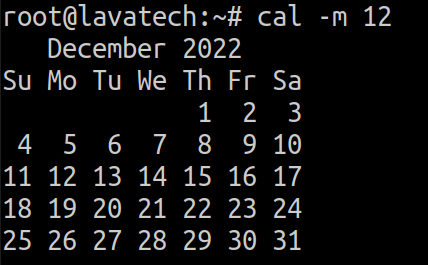
\includegraphics[scale=0.4]{content/chapter2/images/cal2.png}
					\caption{Sample output}
					\label{fig:cal2}
				\end{figure}
				
			
				\item \textbf{-y}: Display entire year.\newline
				Eg: To display calender of year-2022.
			\begin{tcolorbox}[breakable,notitle,boxrule=-0pt,colback=black,colframe=black]
				\color{green}
				\fontdimen2\font=1em
				\# cal -y 2022
				\fontdimen2\font=4pt
			\end{tcolorbox}
			\begin{figure}[h!]
				\centering
				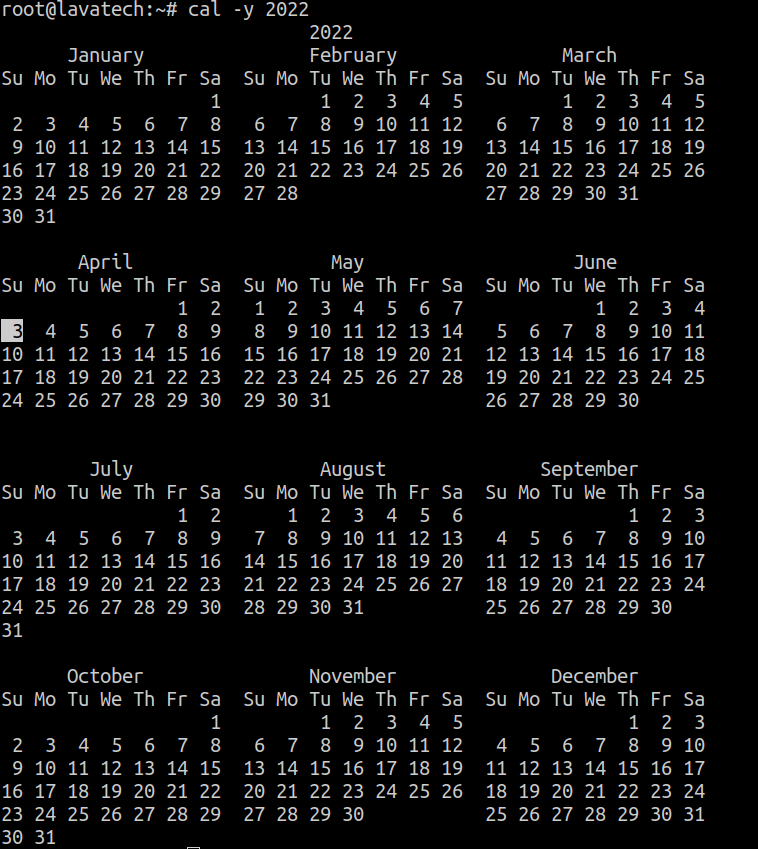
\includegraphics[scale=0.4]{content/chapter2/images/cal3.png}
				\caption{Sample output}
				\label{fig:cal3}
			\end{figure}
			
			\end{itemize}

	\newpage
		\item \textbf{ifconfig}: Display the IP address of server.
		\newline
		Eg:
		\begin{tcolorbox}[breakable,notitle,boxrule=1pt,colback=black,colframe=black]
			\color{green}
			\fontdimen2\font=1em
			\# ifconfig
			\fontdimen2\font=4pt
		\end{tcolorbox}
			\bigskip
			\bigskip		
		\newpage
		\item \textbf{hostname}: Displays the fully qualified name of server.
		\newline
		Eg:
		\begin{tcolorbox}[breakable,notitle,boxrule=1pt,colback=black,colframe=black]
			\color{green}
			\fontdimen2\font=1em
			\# hostname
			\fontdimen2\font=4pt
		\end{tcolorbox}
		\bigskip
		\bigskip
		
		\item \textbf{free}: Displays amount of free and used memory in the system in bytes.
		\newline
			Options with \textbf{free} command:
			\begin{itemize}
				\item \textbf{-k}: Show the output in Kilobytes
				\item \textbf{-m}: Show the output in Megabytes
				\item \textbf{-g}: Show the output in Gegabytes
			\end{itemize}
		Eg:
		\begin{tcolorbox}[breakable,notitle,boxrule=1pt,colback=black,colframe=black]
			\color{green}
			\fontdimen2\font=1em
			\# free 
			\newline
			\# free -k
			\newline
			\# free -m
			\newline
			\# free -g
			\fontdimen2\font=4pt
		\end{tcolorbox}
		
		
		\bigskip
		\bigskip
		\item \textbf{shutdown}: Shutdown the machine immediately or schedule a shutdown using 24 hour format.
		\bigskip
		\begin{tcolorbox}[breakable,notitle,boxrule=1pt,colback=pink,colframe=pink]
			\color{black}
			\fontdimen2\font=1em
			Syntax:  shutdown [options] [time in 24 hour format]
			\fontdimen2\font=4pt
		\end{tcolorbox}
		\bigskip
		\begin{itemize}
			\item Eg: Shutdown immediately -
			\begin{tcolorbox}[breakable,notitle,boxrule=1pt,colback=black,colframe=black]
				\color{green}
				\fontdimen2\font=1em
				\# shutdown -h now
				\newline
				or
				\newline
				\# poweroff
				\fontdimen2\font=4pt
			\end{tcolorbox}
			\item Eg: Reboot the system immediately -
			\bigskip
			\begin{tcolorbox}[breakable,notitle,boxrule=1pt,colback=black,colframe=black]
				\color{green}
				\fontdimen2\font=1em
				\# shutdown -r now
				\newline
				\color{green}
				or
				\newline
				\color{green}
				\# reboot
				\fontdimen2\font=4pt
			\end{tcolorbox}
			\item Eg: Restart OS at specific time, like at 5:30 pm -
			\bigskip
			\begin{tcolorbox}[breakable,notitle,boxrule=1pt,colback=black,colframe=black]
				\color{green}
				\fontdimen2\font=1em
				\# shutdown 17:30
				\fontdimen2\font=4pt
			\end{tcolorbox}
			\item Eg: Shutdown OS at specific time, like at 5:30 pm -
			\bigskip
			\begin{tcolorbox}[breakable,notitle,boxrule=1pt,colback=black,colframe=black]
				\color{green}
				\fontdimen2\font=1em
				\# shutdown -h 17:30
				\fontdimen2\font=4pt
			\end{tcolorbox}
		\end{itemize}

		\bigskip
		\bigskip
		

		\item \textbf{which}: Shows the full path of the command.
		\bigskip
		\begin{tcolorbox}[breakable,notitle,boxrule=1pt,colback=pink,colframe=pink]
			\color{black}
			\fontdimen2\font=1em
			Syntax: which command\_name
			\fontdimen2\font=4pt
		\end{tcolorbox}
		Eg:
		\bigskip
		\begin{tcolorbox}[breakable,notitle,boxrule=1pt,colback=black,colframe=black]
			\color{green}
			\fontdimen2\font=1em
			\# which cal
			\newline
			\color{white}
			/usr/bin/cal
			\fontdimen2\font=4pt
		\end{tcolorbox}

		
		\bigskip
		\bigskip
		
		\item \textbf{whereis}: Locate the binary, source, and manual page files for a command.
		\bigskip
		\begin{tcolorbox}[breakable,notitle,boxrule=1pt,colback=pink,colframe=pink]
			\color{black}
			\fontdimen2\font=1em
			Syntax: whereis command\_name
			\fontdimen2\font=4pt
		\end{tcolorbox}
		Eg:
		\bigskip
		\begin{tcolorbox}[breakable,notitle,boxrule=1pt,colback=black,colframe=black]
			\color{green}
			\fontdimen2\font=1em
			\# whereis cal
			\newline
			\color{white}
			cal: /usr/bin/cal /usr/share/man/man1/cal.1.gz
			\fontdimen2\font=4pt
		\end{tcolorbox}
		\bigskip
		\bigskip
		

		\item \textbf{sleep}: Suspends the shell by making it inactive for specified seconds.
		\begin{tcolorbox}[breakable,notitle,boxrule=1pt,colback=pink,colframe=pink]
			\color{black}
			\fontdimen2\font=1em
			Syntax: sleep seconds
			\fontdimen2\font=4pt
		\end{tcolorbox}
		Eg:
		\bigskip
		\begin{tcolorbox}[breakable,notitle,boxrule=1pt,colback=black,colframe=black]
			\color{green}
			\fontdimen2\font=1em
			\# sleep 10
			\fontdimen2\font=4pt
		\end{tcolorbox}
		\bigskip
		\bigskip	

				
		\item \textbf{history}: Shows last few commands fired by the current user.
		\newline
		Eg:
		\begin{figure}[h!]
			\centering
			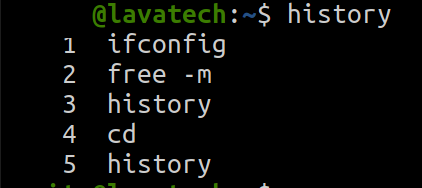
\includegraphics[scale=.4]{content/chapter2/images/history.png}
			\caption{history command output}
			\label{fig:h6}
		\end{figure}
	\newline
		Options using \textbf{history} command:
		\newline
		\textbf{-c}: Clear the history.
			\begin{tcolorbox}[breakable,notitle,boxrule=1pt,colback=pink,colframe=pink]
				\color{black}
				\fontdimen2\font=1em
				Syntax:  history -c
				\fontdimen2\font=4pt
			\end{tcolorbox}
		Shortcuts using \textbf{history} command:
		\newline
		\textbf{!}: Used to repeat the command executed in past, using it's history number.
		\begin{tcolorbox}[breakable,notitle,boxrule=1pt,colback=pink,colframe=pink]
			\color{black}
			\fontdimen2\font=1em
			Syntax:  !history-no
			\fontdimen2\font=4pt
		\end{tcolorbox}
		Eg:
		\begin{figure}[h!]
			\centering
			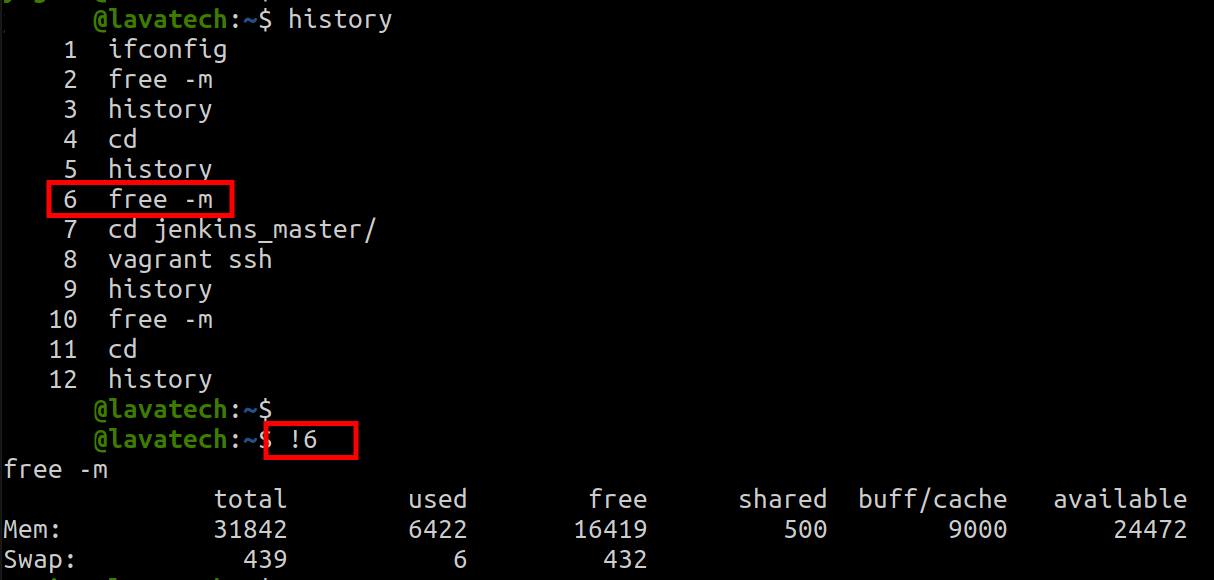
\includegraphics[scale=.2]{content/chapter2/images/history2.png}
			\caption{history command output}
			\label{fig:h88}
		\end{figure}

		\newpage
		\item \textbf{ping}: Used to check if a machine is reachable or not on the network.
		\newline
		\begin{tcolorbox}[breakable,notitle,boxrule=1pt,colback=pink,colframe=pink]
			\color{black}
			\fontdimen2\font=1em
			Syntax:  ping ip-address/hostname
			\fontdimen2\font=4pt
		\end{tcolorbox}
		Eg:
		\begin{tcolorbox}[breakable,notitle,boxrule=1pt,colback=black,colframe=black]
			\color{green}
			\fontdimen2\font=1em
			\# ping 192.168.1.0
			\newline
			\# ping www.google.com
			\fontdimen2\font=4pt
		\end{tcolorbox}
		\bigskip
		\begin{tcolorbox}[breakable,notitle,boxrule=1pt,colback=yellow,colframe=yellow]
			\color{black}
			Note: Ping works continuously until ctrl+c is pressed.
		\end{tcolorbox}
		\bigskip
		Options with \textbf{ping} command:
		\newline
		\textbf{-cN}: Send data N number of times using ping command.	
		\newline
		Eg:
		\begin{figure}[h!]
			\centering
			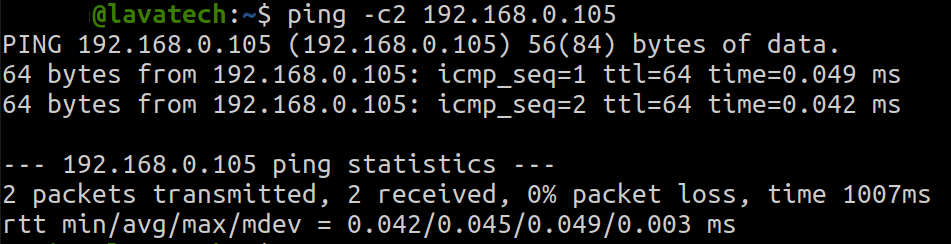
\includegraphics[scale=.35]{content/chapter2/images/ping.png}
			\caption{ping command output}
			\label{fig:h1}
		\end{figure}
		\bigskip
		\bigskip
		\item \textbf{man}: Display manual pages of commands.
		\bigskip
		\begin{tcolorbox}[breakable,notitle,boxrule=1pt,colback=pink,colframe=pink]
			\color{black}
			\fontdimen2\font=1em
			Syntax: man command\_name
			\fontdimen2\font=4pt
		\end{tcolorbox}
		Eg:
		\bigskip
		\begin{tcolorbox}[breakable,notitle,boxrule=1pt,colback=black,colframe=black]
			\color{green}
			\fontdimen2\font=1em
			\# man date
			\fontdimen2\font=4pt
		\end{tcolorbox}
		Options with \textbf{man} command:
		\newline
		\textbf{-k}: Search for man page using keyword
		\begin{tcolorbox}[breakable,notitle,boxrule=1pt,colback=pink,colframe=pink]
			\color{black}
			\fontdimen2\font=1em
			Syntax: man -k keyword
			\fontdimen2\font=4pt
		\end{tcolorbox}
		Eg:
		\begin{figure}[h!]
			\centering
			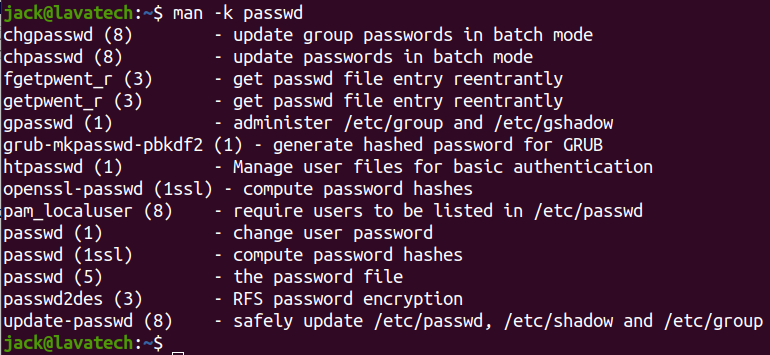
\includegraphics[scale=.5]{content/chapter2/images/man2.png}
			\caption{Command Prompt}
			\label{fig:command_prompt2}
		\end{figure}

	
		\bigskip
		\bigskip


		\item \textbf{whatis}: Provides very brief descriptions of the command.
		\bigskip
		\begin{tcolorbox}[breakable,notitle,boxrule=1pt,colback=pink,colframe=pink]
			\fontdimen2\font=1em
			\color{black}
			Syntax: whatis command\_name
			\fontdimen2\font=4pt
		\end{tcolorbox}
		Eg:
		\bigskip
		\begin{tcolorbox}[breakable,notitle,boxrule=1pt,colback=black,colframe=black]
			\fontdimen2\font=1em
			\color{green}
			\# whatis cal
			\color{white}
			\newline
			cal (1)              - displays a calendar and the date of Easter
			\fontdimen2\font=4pt
		\end{tcolorbox}
		
		\bigskip
		\bigskip
		
		\item \textbf{echo}: Display custom message.
		\bigskip
		\begin{tcolorbox}[breakable,notitle,boxrule=1pt,colback=pink,colframe=pink]
			\color{black}
			\fontdimen2\font=1em
			Syntax: echo "message"
			\fontdimen2\font=4pt
		\end{tcolorbox}
		Eg:
		\bigskip		
		\begin{tcolorbox}[breakable,notitle,boxrule=1pt,colback=black,colframe=black]
			\color{green}
			\fontdimen2\font=1em
			\# echo "lavatech technology training institute"
			\fontdimen2\font=4pt
		\end{tcolorbox}
		Executing command along with custom message:
		\begin{tcolorbox}[breakable,notitle,boxrule=1pt,colback=pink,colframe=pink]
			\color{black}
			\fontdimen2\font=1em
			Syntax: echo "message \$(command)"
			\newline
			or
			\newline
			Syntax: echo "message `command`"
			\fontdimen2\font=4pt
		\end{tcolorbox}
		Eg:
		\bigskip		
		\begin{tcolorbox}[breakable,notitle,boxrule=1pt,colback=black,colframe=black]
			\color{green}
			\fontdimen2\font=1em
			\# echo "lavatech technology training institute, date: \$(date)"
			\newline
			\# echo "lavatech technology training institute, date: `date`"
			\fontdimen2\font=4pt
		\end{tcolorbox}
		\bigskip
		\bigskip	
		
		\item \textbf{alias}: Sets an alias (similar to nickname) for a command.
		\bigskip
		\begin{tcolorbox}[breakable,notitle,boxrule=1pt,colback=pink,colframe=pink]
			\color{black}
			\fontdimen2\font=1em
			Syntax: alias 'shortcutname=command'
			\fontdimen2\font=4pt
		\end{tcolorbox}
		Eg:
		\bigskip
		\begin{tcolorbox}[breakable,notitle,boxrule=1pt,colback=black,colframe=black]
			\color{green}
			\fontdimen2\font=1em
			\# alias 'cls=clear'           
			\fontdimen2\font=4pt
		\end{tcolorbox}
		\bigskip
		\bigskip	
		
		\item \textbf{unalias}: Remove an alias.
		\bigskip
		\begin{tcolorbox}[breakable,notitle,boxrule=1pt,colback=pink,colframe=pink]
			\color{black}
			\fontdimen2\font=1em
			Syntax: unalias shortcutname
			\fontdimen2\font=4pt
		\end{tcolorbox}
		Eg:
		\bigskip
		\begin{tcolorbox}[breakable,notitle,boxrule=1pt,colback=black,colframe=black]
			\color{green}
			\fontdimen2\font=1em
			\# unalias cls
			\fontdimen2\font=4pt
		\end{tcolorbox}
		\bigskip
		\bigskip	
		

		
	\end{enumerate}
	
\end{flushleft}

\newpage

